\documentclass[10pt,twocolumn]{article}
\usepackage[a4paper, top=2cm, bottom=2cm, left=2cm, right=2cm]{geometry}
\usepackage{epsfig}
\usepackage[font=footnotesize]{caption}
\usepackage{amsmath,graphicx,psfrag,pstcol}
\graphicspath{{/Users/ranshanzi/Documents/VSCode/GG2/reports/results}}
\usepackage{xcolor}
\usepackage{subcaption}
\usepackage{tipa}
\usepackage{listings}
\usepackage{xcolor} 
\lstdefinestyle{mypython}{
    language=Python,
    basicstyle=\ttfamily\footnotesize,
    keywordstyle=\color{blue},
    commentstyle=\color{gray},
    stringstyle=\color{orange},
    showstringspaces=false,
    breaklines=true,
    tabsize=4
}
\usepackage{titlesec}
\titleformat*{\section}{\normalsize\bfseries}
\titleformat*{\subsection}{\small\bfseries}
\titleformat*{\subsubsection}{\small\bfseries}
\titleformat*{\paragraph}{\footnotesize\bfseries}

\begin{document}
\title{\vspace{-2cm}\bfseries \Large GG2: CT Reconstruction and Visualisation\\[0.5em] \normalsize Interim Report}
\author{\small Shanzi (Monica) Ran (sr2021)\\}
\date{\small \today}
\maketitle

\section{Introduction}
This report documents the process of project GG2, which includes attemps and experiments in simulating the functions of a CT scanner. The project is build upon the provided codebase and progressively implements the generation, attenuation, and reconstruction of X-ray data, as well as visualising more complex functionalities like the noise to achieve more realistic simulation.

\section{X-ray Generation, Scattering, and Detection}
\subsection{Fundamental properties of X-rays}
X-rays, widely used in medical imaging, are high-energy electromagnetic radiation produced by bombarding target metals, yielding a polychromatic energy spectrum with characteristic peaks that can be partially suppressed using filters.

X-ray interactions with matter occur mainly via photoelectric absorption at low energies and Compton scattering or pair production at higher energies; lower-energy Rayleigh scattering is negligible in the CT range relevant to this project.

X-ray intensity, proportional to photon count, can be measured using scintillators, which convert X-rays to visible light \cite{KRAMAR19992467}. Comparing attenuation across materials and depth reveal useful information about the internal structure and properties of materials. Due to the probabilistic nature of X-ray interactions, collimators are used at the source and detector to reduce scatter, though high-energy scattering may still cause artefacts, as discussed later.

\subsection{Material Linear Attenuation Coefficient}
\begin{figure}[htbp]
    \centering
    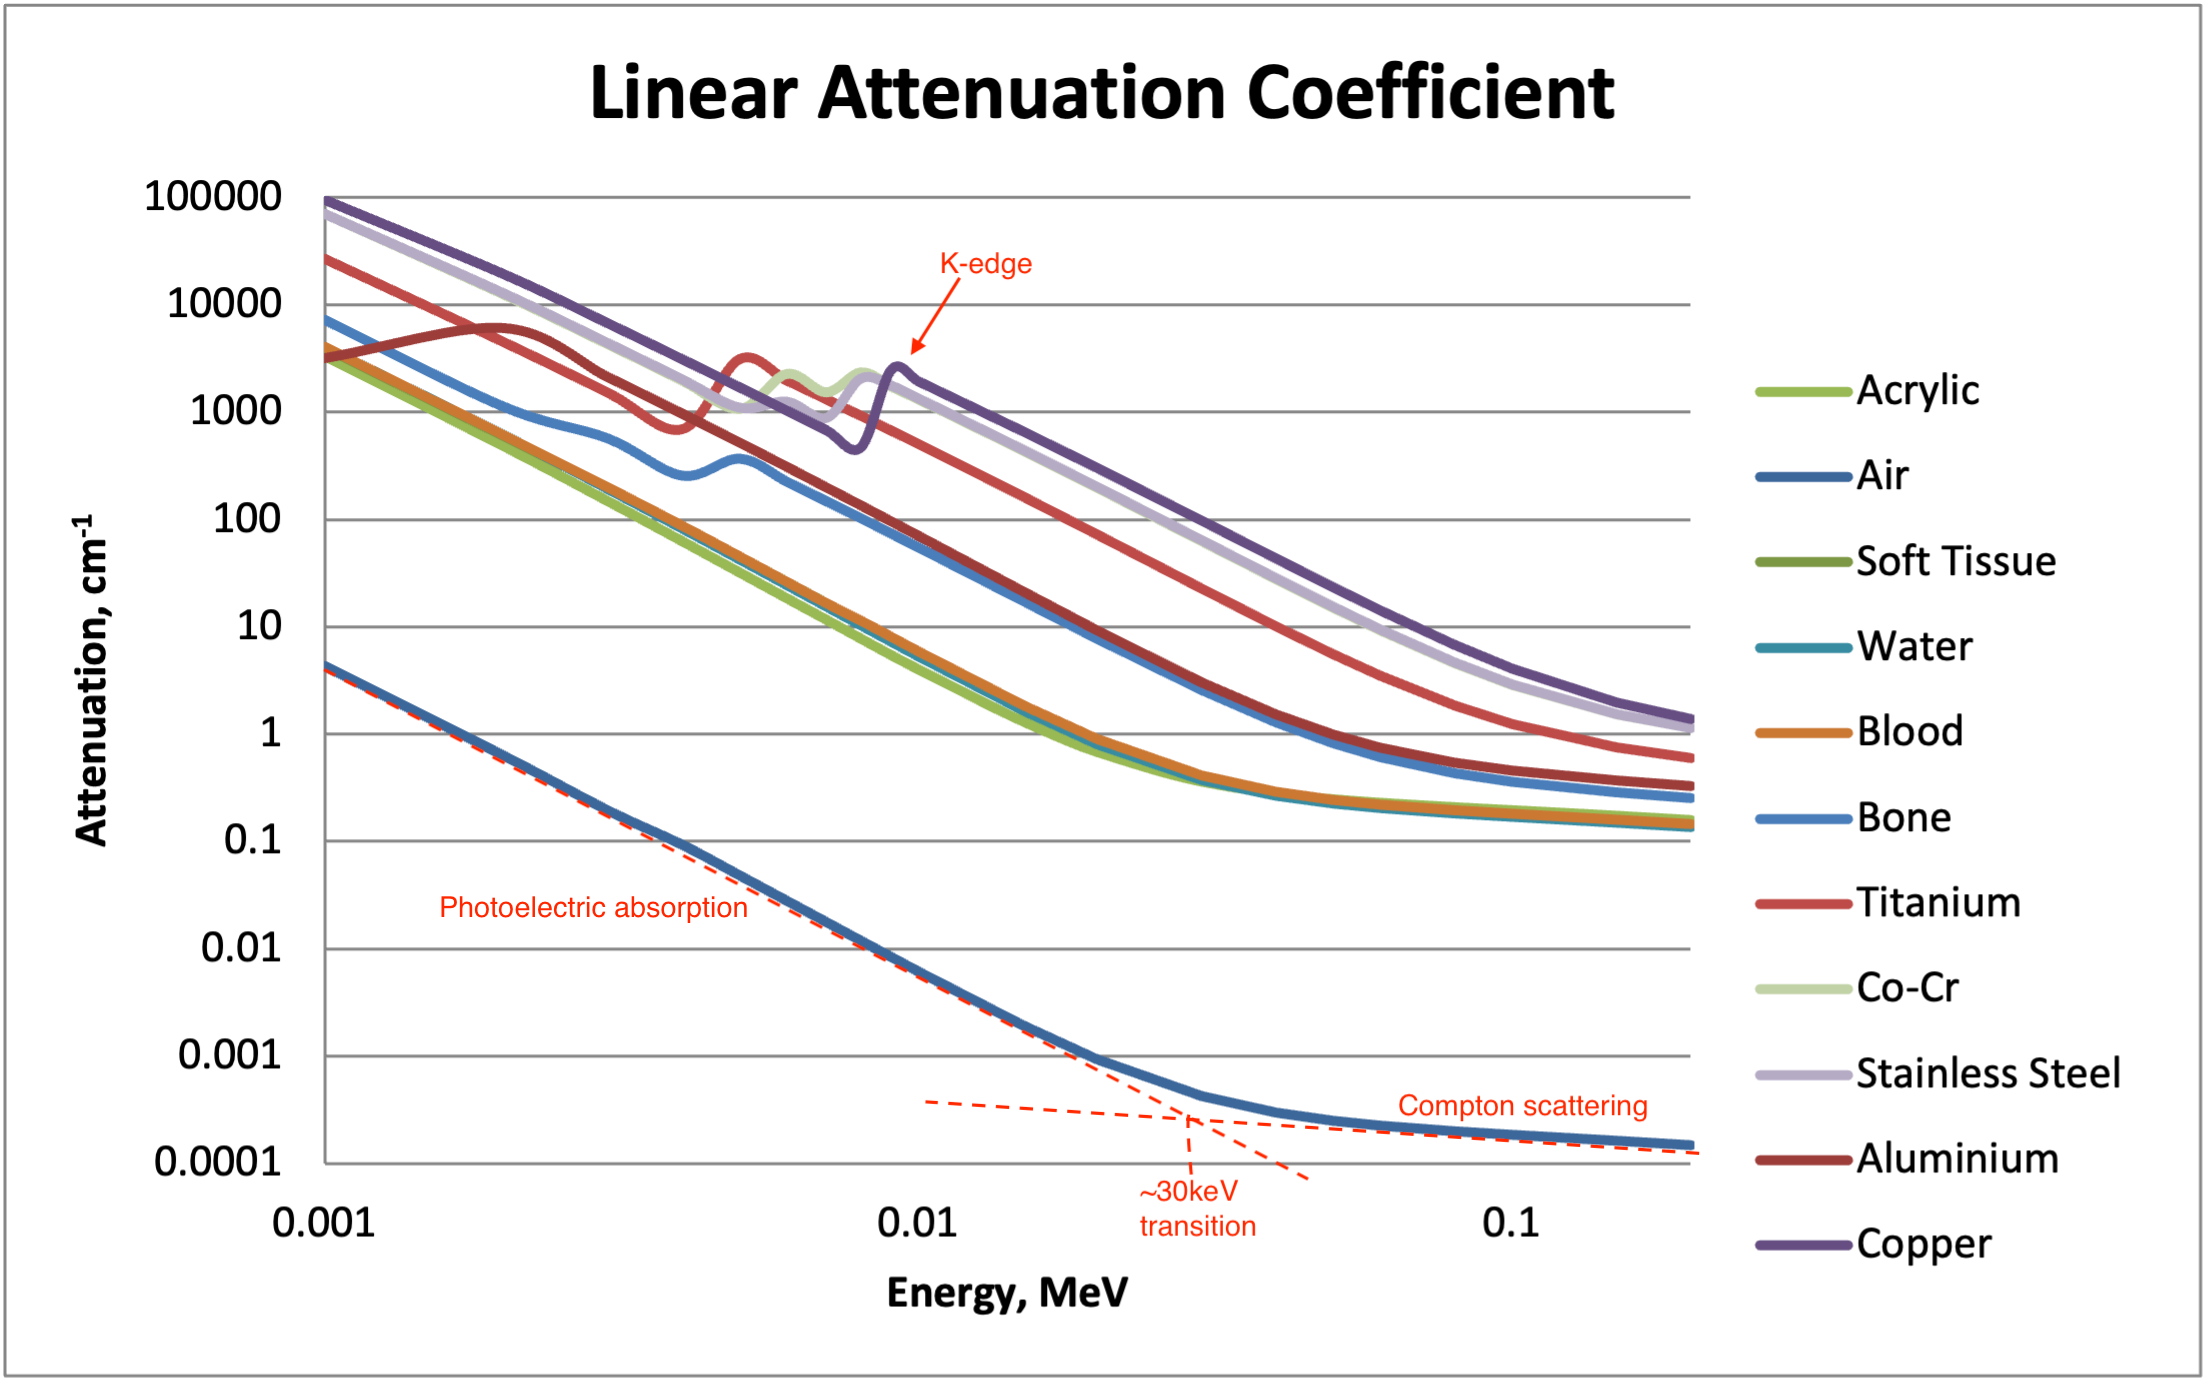
\includegraphics[width=\linewidth]{annotated_mu.png}
    \caption{Linear attenuation coefficient $\mu$ against X-ray energy for various materials}
    \label{fig:mu}
\end{figure}

The interaction of ionizing X-ray radiation with matter is often characterized by the macroscopic linear attenuation coefficient $\mu$, which is determined both by the material and energy of the X-ray. 
At low energy (50 keV or less \cite{transition}) photoelectric absorption is dominant, while Compton scattering is more prominent as energy increases. 

The atomic number $Z$ of the material is significant in determining its attenuation behaviour. It can be approximated from the graph supplied in the handout that $\mu$ increases proprotional to $Z^3$. For higher $Z$, K- and L- absorption edge discontinuities are present as attenuation increases sharply at energies coinciding with the binding energies of electrons for each element \cite{Seibert3}.

\subsection{Simulating X-ray Attenuation}
\vspace{-2em}
\begin{figure}[htbp]
    \centering
    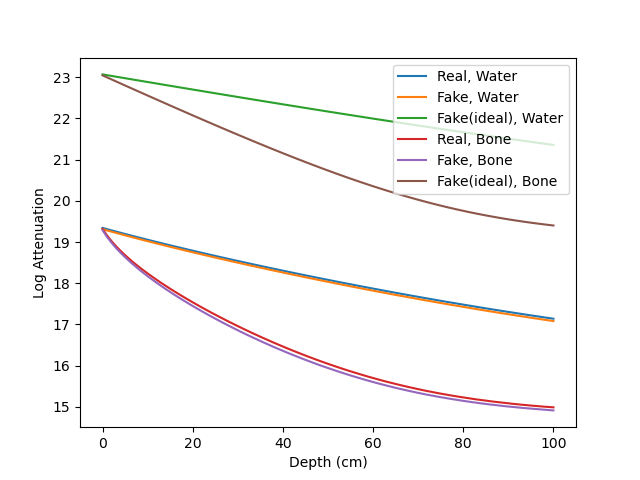
\includegraphics[width=\linewidth]{attenuation.png}
    \caption{Simulated X-ray attenuation for different materials and different sources at 100 keV, where \textit{Real} is 100kVp source with 2mm Aluminium filter that has polychromatic spikes due to bremsstrahlung, \textit{Fake} is source generated using \texttt{fake\_source}, and \textit{Fake(ideal)} is single-energy fake source.}
    \label{fig:attenuation}
\end{figure}

As stated by the Beer-Lambert law, the logarithm of intensity and depth should ideally follow a linear relationship. 
Fig~\ref{fig:attenuation} confirms this linearity for ideal single-energy sources, but real sources exhibit more non-linearity due to the polychromatic nature of the X-ray beam. Materials with higher $Z$ like bone show more non-linearity than materials like water as they have more interaction with the X-ray beam. For each material, more non-linearity is observed at smaller depths, which is likely because a relatively small portion of the beam is involved in the interactions.

\section{CT Scanning and Sinogram}
\subsection{Simulating CT Scanning}
\paragraph{Sinogram for Different Phantom Shapes}

\begin{figure}[htbp]
    \centering
    \begin{subfigure}[b]{0.3\linewidth}
        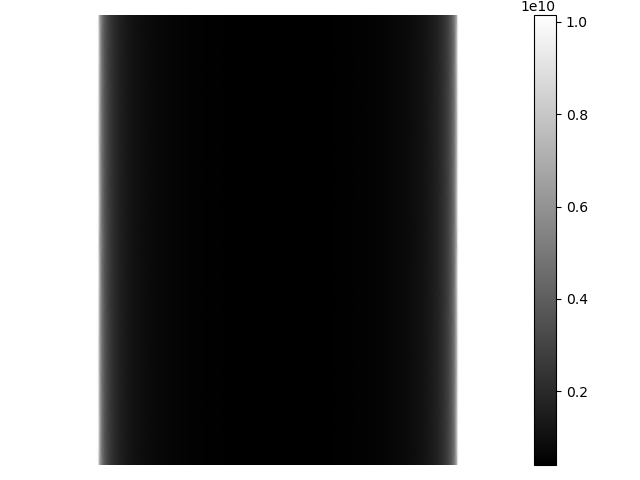
\includegraphics[width=\linewidth]{sinogram_1.png}
        \caption{}
    \end{subfigure}
    \begin{subfigure}[b]{0.3\linewidth}
        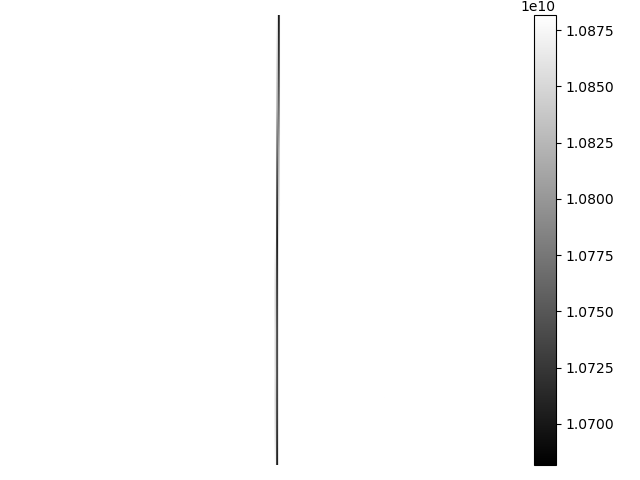
\includegraphics[width=\linewidth]{sinogram_2.png}
        \caption{}
    \end{subfigure}
    \begin{subfigure}[b]{0.3\linewidth}
        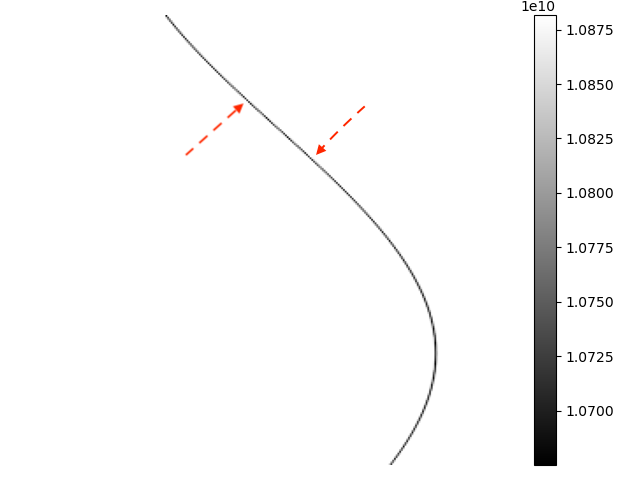
\includegraphics[width=\linewidth]{sinogram_3.png}
        \caption{}
    \end{subfigure}

    \begin{subfigure}[b]{0.3\linewidth}
        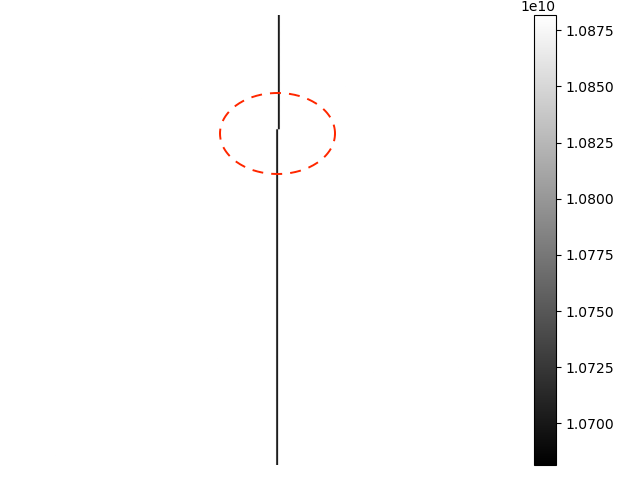
\includegraphics[width=\linewidth]{sinogram_2_nn.png}
        \caption{}
    \end{subfigure}
    \begin{subfigure}[b]{0.3\linewidth}
        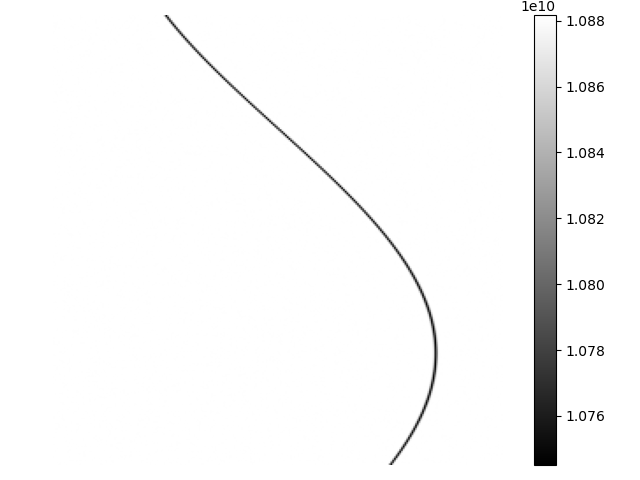
\includegraphics[width=\linewidth]{sinogram_3_cubic.png}
        \caption{}
    \end{subfigure}
    \caption{Sinograms for various phantom shapes, which is a 2D dataset of $p(r, \theta)$ stacked for each angle scanned. (a)Disk phantom. (b)Point attenuator at the centre of the scan. (c)Point attenuator off-centre. (Linear interpolation, with small discontinuities marked) (d)Point attenuator at centre with nearest-neighbour interpolation. (discontinuity marked)(e)Point attenuator off-centre with cubic interpolation.}
    \label{fig:sinogram_shapes}
\end{figure}
The sinograms in Fig~\ref{fig:sinogram_shapes} show the projection data for simple phantom shapes without calibration for air attenuation. 
These results confirm that the \texttt{ct\_scan} function produces sinograms as expected, where a centrally-located circular disk has same attenuation from all scanning angles, and the off-centred point attenuator gives different attenuation as the depth changes with angle.

\paragraph{Number of Angles}
The number of angles used in the CT scan controls the angular sampling of the sinogram, which directly affects angular resolution of generated sinogram and subsequent reconstructions. 

\paragraph{Interpolation Methods}
Interpolation of the depth field is necessary as the rotating X-ray direction is in general not aligned with the pixel axes. Fig~\ref{fig:sinogram_shapes} also shows the effect of different interpolation methods of the phantom depths on the sinogram. It is clear that although a lower order interpolation reduces computation, it may introduce discontinuties in values of the projection data even for simple shapes.

\subsection{Sinogram Calibration}
\begin{figure}[htbp]
    \centering
    \begin{subfigure}[b]{0.44\linewidth}
        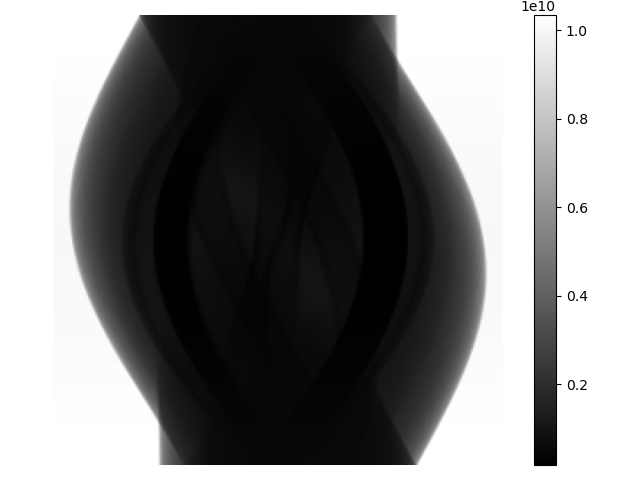
\includegraphics[width=\linewidth]{sinogram_4.png}
        \caption{Original}
    \end{subfigure}
    \hspace{0.03\linewidth}
    \begin{subfigure}[b]{0.44\linewidth}
        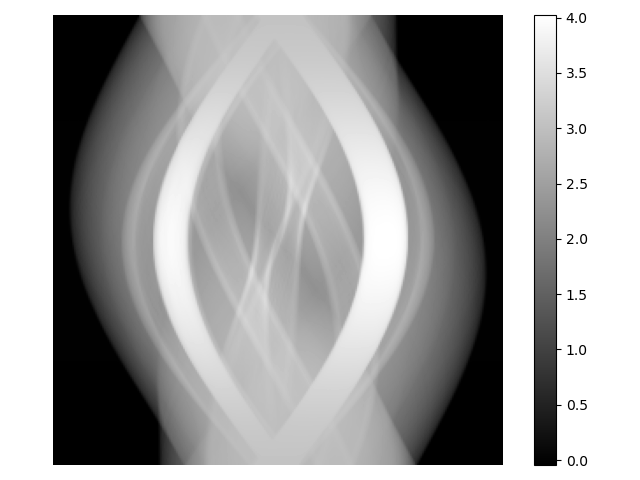
\includegraphics[width=\linewidth]{sinogram_calibrated.png}
        \caption{Calibrated}
    \end{subfigure}
    \caption{Sinograms of the bilateral hip replacement scan (a)before and (b)after calibration using air attenuation.}
    \label{fig:sinogram_calibration}
\end{figure}
Calibration of the sinogram using a known material (air) that covers the whole field of scan is essential to convert the original intensity profile (like Fig~\ref{fig:sinogram_shapes}) to total attenuation. 
Fig~\ref{fig:sinogram_calibration} shows an example of correctly calibrated sinogram.

\section{Reconstructing Cross-sectional Data}
\subsection{Fundamentals of Filtered Back-Projection (FBP)}
FBP is a powerful method for reconstructing cross-sectional linear attenuation data $\mu(x,y)$ form the measured dataset of total intensity attenuations $p(r,\theta)$. 
It repeats for each angle $\theta$ the polar 2D inverse Fourier transform of the projection data convolved with a ramp filter, which is implemented as a discrete bandlimited Ram-Lak filter. FBP improves the reconstruction quality by avoiding interpolation in 2D cartesian space.
FBP introduced in this report is based on the parallel-beam geometry implemented in the project, while other complexities may be added for more advanced generations of CT.

\subsection{Ramp Filtering}
\begin{figure}[htbp]
    \centering
    \begin{subfigure}[b]{0.44\linewidth}
        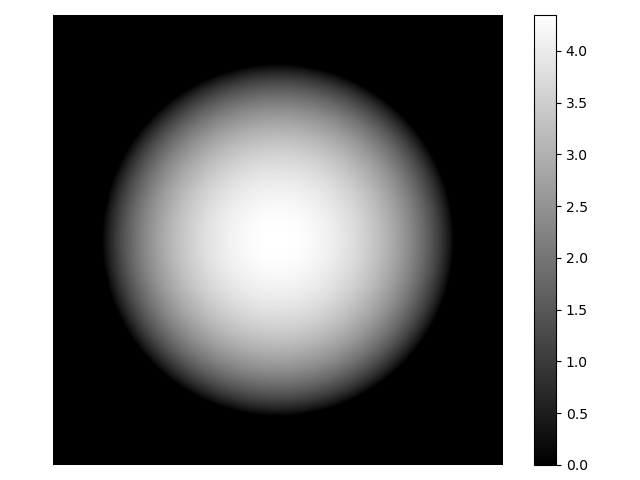
\includegraphics[width=\linewidth]{reconstruct_no_filter_disk.png}
        \caption{No Filter}
    \end{subfigure}
    \begin{subfigure}[b]{0.44\linewidth}
        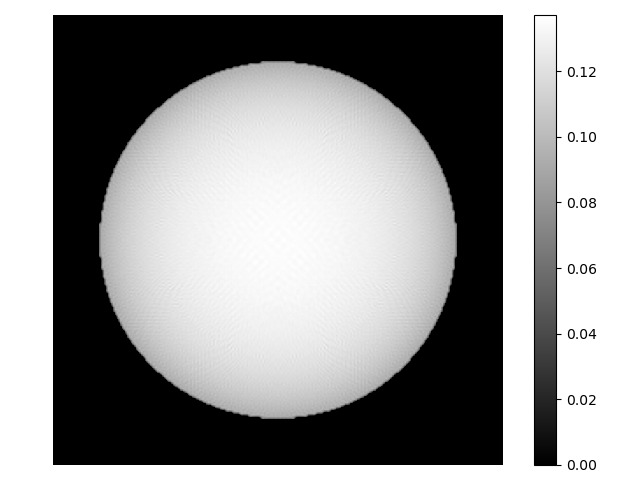
\includegraphics[width=\linewidth]{reconstruct_filter_disk.png}
        \caption{Filtered}
    \end{subfigure}
    \caption{Reconstructed disk phantom using FBP without and with ramp filter in (c), where filtering removes blurring artefacts.}
    \label{fig:filter_reconstruction}
\end{figure}
Fig~\ref{fig:filter_reconstruction} shows the reconstructed phantoms using FBP without and with ramp filtering. It is clear that the ramp filter improves reconstruction quality by amplifying high-frequency components, thus reduce blurring \cite{Lyra_Ploussi_2011}.
\begin{figure}[htbp]
    \centering
    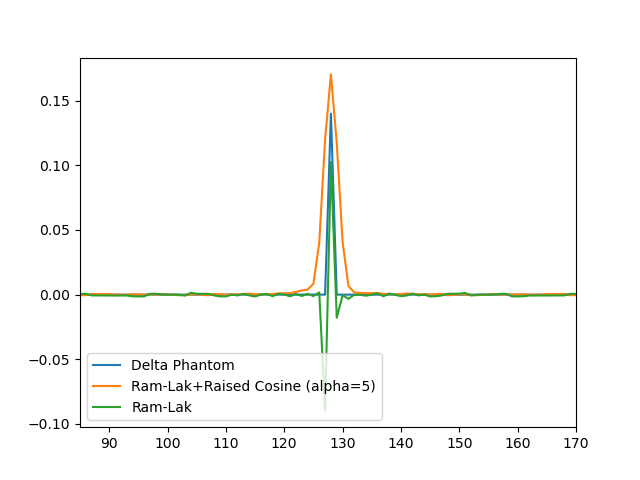
\includegraphics[width=\linewidth]{filter_impulse.png}
    \caption{Impulse response of the Ram-Lak filter with and without raised cosine smoothing.}
    \label{fig:filter_impulse}
\end{figure}

\paragraph{Impulse Response of Ramp Filter}
The Ram-Lak filter is implemented in discrete frequency space by approximating results from \cite{6940329} to preserve low-frequency information and prevent aliasing.
Fig~\ref{fig:filter_impulse} shows the scaled response of the Ram-Lak filter to a simulated impulse at the centre of the image. Due to the discretisation and approximation of the filter implimentation, the response is not perfectly bandlimited and symmetric as expected for ideal Ram-Lak filters.
It is also observed from the impulse response that the raised cosine filter successfully smooths the high-frequency fluctuations in original filter response.

\subsection{Simulating CT Reconstruction}
\paragraph{Number of Angles}
\begin{figure}[htbp]
    \centering
    \begin{subfigure}[b]{0.3\linewidth}
        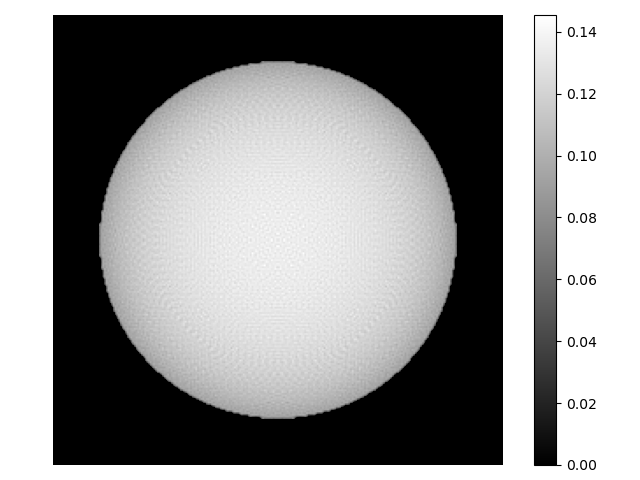
\includegraphics[width=\linewidth]{angle_128.png}
        \caption{}
    \end{subfigure}
    \begin{subfigure}[b]{0.3\linewidth}
        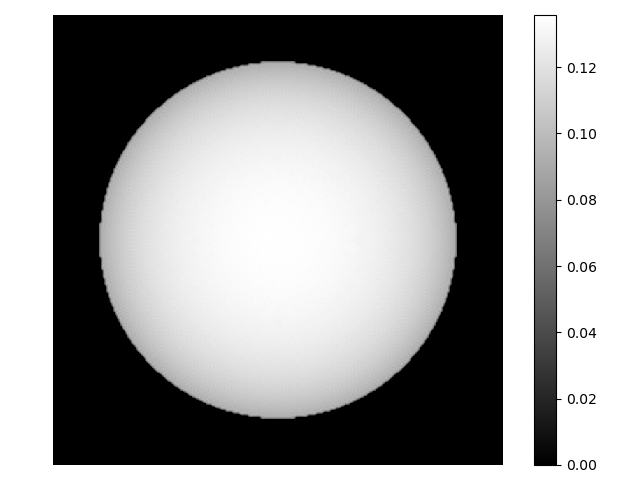
\includegraphics[width=\linewidth]{angle_320.png}
        \caption{}
    \end{subfigure}
    \begin{subfigure}[b]{0.3\linewidth}
        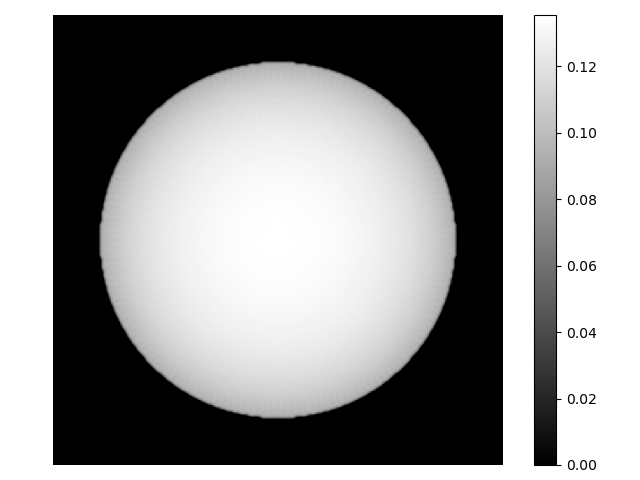
\includegraphics[width=\linewidth]{angle_2_160.png}
        \caption{}
    \end{subfigure}
    \centering
    \begin{subfigure}[b]{0.3\linewidth}
        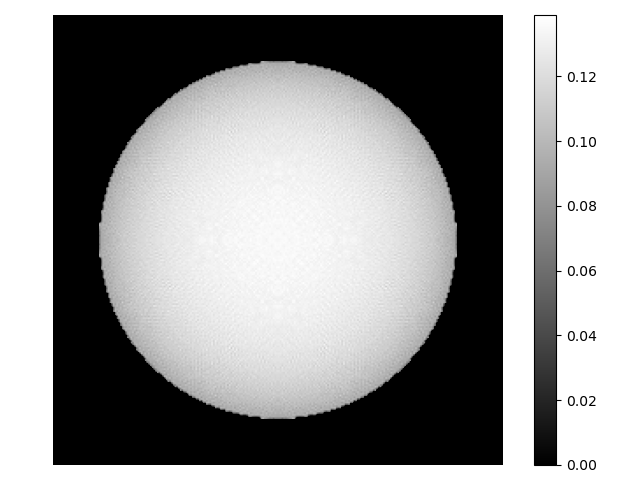
\includegraphics[width=\linewidth]{nearest.png}
        \caption{}
    \end{subfigure}
    \begin{subfigure}[b]{0.3\linewidth}
        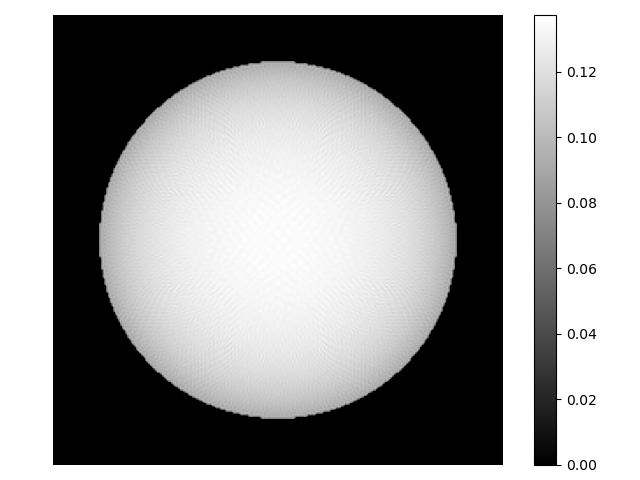
\includegraphics[width=\linewidth]{cubic.png}
        \caption{}
    \end{subfigure}
    \begin{subfigure}[b]{0.3\linewidth}
        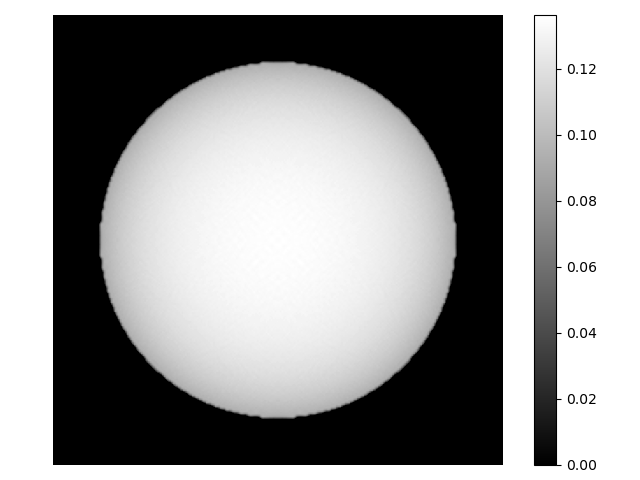
\includegraphics[width=\linewidth]{nearest_2.png}
        \caption{}
    \end{subfigure}
    \caption{Reconstructed disk phantom with different number of angles. (a) 128 angles, (b) 320 angles, (c) 160 angles with order $\alpha=2$ raised cosine filter, (d) nearest-neighbour interpolation in FBP, (e) cubic interpolation in FBP, and (f) nearest-neightbour interpolation with order $\alpha=2$ raised cosine.}
    \label{fig:angle}
\end{figure}

Similar to the forward projection, the number of angles used in FBP directly affects the quality of reconstructed image as it determines angular sampling. If the number of angles is too low, the reconstruction from under-sampled data will suffer from visible artefacts.
Experimenting with different numbers of angles, it is found that 320 angles is sufficient to remove most granularity in the reconstructed image with minimum compulation.
It is also observed that a smaller number of angles is required to achieve similar quality for phantoms generated with higher resolution, as details are inherently more accurate.

\paragraph{Interpolation Methods}
It is also investigated how different interpolation methods in the back-projected $\mu(x, y)$ affects visualisation quality and image resolution. For the fixed pixel and angular resolution, nearest-neighbour interpolation produces significant rough edges and granular artefacts, while cubic interpolation may also introduce artefacts which likely originates from numerical instabilities.
Linear interpolation gives a reasonable balance between computation and quality for each phantom tested.

\subsection{Raised-cosine Filter}
As shown by the impulse reponse in Fig~\ref{fig:filter_reconstruction}, the Ram-Lak filter has a sharp cut-off at the Nyquist frequency, which may introduce ringing artefacts in the reconstructed image.
To address this, a raised cosine filter is applied to smooth the Ram-Lak filter response with tunable order.

Applying the raised cosine filter smooths the reconstructed image and reduces Gibbs ringing artefacts at fixed angular sampling\cite{JEZZARD2000425}, which allows for similar quality with fewer angle scans.
For example, with order $\alpha=2$ raised cosine smoothing, the reconstructed image shown in Fig~\ref{fig:angle} of 160 scans achieves similar quality as using 320 scans without the raised-cosine. This allows for better reconstruction at lower computational cost.

The raised cosine filter also reduces the effect of interpolation accuracy on the reconstruction, as the filter smooths out the high-frequency components caused by discontinuities in interpolated data. This enables lower-order interpolation methods like nearest-neighbour to achieve similar quality as higher-order methods like cubic interpolation.

\section{Refinement for Realistic CT Simulation}
In order to more accurately simulate the performance of a real CT scanner, several refinements are introduced, including statistical and scatter noise, beam hardening correction, and Hounsfield Units (HU) calibration.
This part of the project is based on a cooperative split of the work, where I focus on simulating noise in the scanning process.

\subsection{Noise in CT Simulation}
\subsubsection{Three Types of Noise}
\paragraph{Statistical Noise}
Due to the stochastic nature of particle interactions, quantum noise is present in both the source and transmission of X-rays, which can be modelled as a Poisson distribution that the probability of measuring $n$ photons when mean is $\lambda$ is given by $P(n|\lambda)=(e^{-\lambda}\lambda^n)/n!$\cite{Suetens_2009}. This is achieved using the provided (or generated) photon count as the expected value.
This results in slight variations in the measured intensity as the overall number of photons and reconstructed image is not affected significantly.

\paragraph{Background Radiation}
Background environmental radiation introduces a constant offset to the measured intensity, which is also modelled as a Poisson distribution. The background radiation is low in value compared to the CT diagnostic dosage, and is modelled as $0.1\%$ of the peak X-ray energy of the source for reasonable visible distortion (observed as blurry edges and rescaled intensity).

\paragraph{Scatter Noise}
Scattering of X-rays results in a smooth increase in detected intensity that amounts up to $30\%$ of the total incident energy, which leads to potential underestimation of the attenuation and reduced level of contrast\cite{Suetens_2009}. 
Although collimators installed at detectors, strongly attenuating objects, like bones and metallic implants, still cause significant beam hardening artefacts in the form of streaks\cite{https://doi.org/10.1118/1.4709599}. 
The scatter noise is modelled as a Possion distribution, where the mean is the number of detected photons scaled differently by different materials, with higher scale $s$ for strongly attenuating materials like bone and metals. 

For each of the three noise types, the Poisson distribution is approximated by a Gaussian distribution $\mathcal{N}(\lambda, \lambda)$ when $\lambda$ exceeds $1000$ for simplicity.

\subsubsection{Noise and \texttt{mas} X-ray Exposure}
\begin{figure}[htbp]
    \centering
    \begin{subfigure}[b]{0.3\linewidth}
        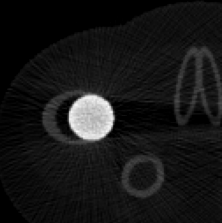
\includegraphics[width=\linewidth]{test_noise_mas_10.png}
        \caption{}
    \end{subfigure}
    \begin{subfigure}[b]{0.3\linewidth}
        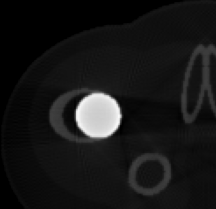
\includegraphics[width=\linewidth]{test_noise_mas_10000.png}
        \caption{}
    \end{subfigure}
    \begin{subfigure}[b]{0.3\linewidth}
        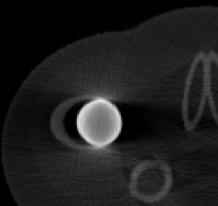
\includegraphics[width=\linewidth]{test_noise_scale_03.png}
        \caption{}
    \end{subfigure}
    \caption{Reconstructed images of bilateral hip replacement phantom. (a) with low mAs value of 10, (b) with high mAs value of 10000, (c) with larger pixel size 0.3mm}
    \label{fig:noise_mas}
\end{figure}
Fig~\ref{fig:noise_mas} shows the reconstructed images under different \texttt{mas} values, which is the product of X-ray tube current and exposure time.
As expected, higher mAs results in a clearer image with less noise, while the noise is more pronounced in the low \texttt{mas} case as streaking artefacts are more visible. This is because when fewer photons are generated per scan, the quantum(statistical) noise will dominate. 
However, increasing the mAs value only changes noise behaviour, and does not generally affect overall contrast of the image.

As shown in the reconstructed images, when a very high attenuation mateiral is present, the X-ray is almost completely blocked, which leads to severe streaking behind the material and details are further obscured.
The physical size of the pixel also affects the severity of streaking artefects, as larger pixels will result in more attenuation and scattering noises simultaneously. The reconstructed image under larger pixel size shows more severe streaking artefects as well as bean hardening artefacts.

\subsubsection{Noise Compensation by Raised Cosine Filter}
\begin{figure}[htbp]
    \centering
    \begin{subfigure}[b]{0.46\linewidth}
        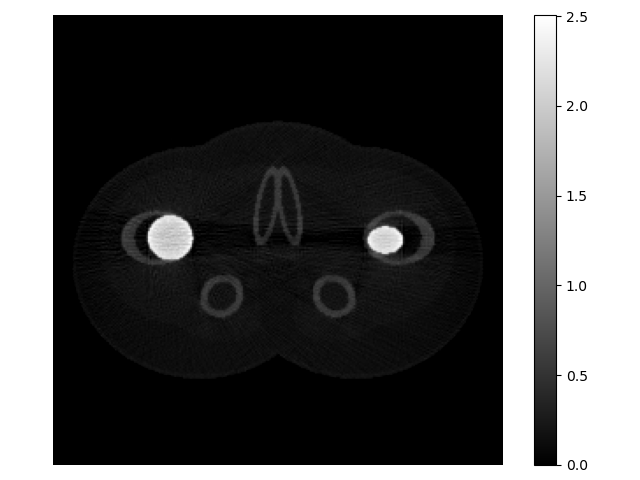
\includegraphics[width=\linewidth]{test_noise_no_ramlak.png}
        \caption{}
    \end{subfigure}
    \begin{subfigure}[b]{0.46\linewidth}
        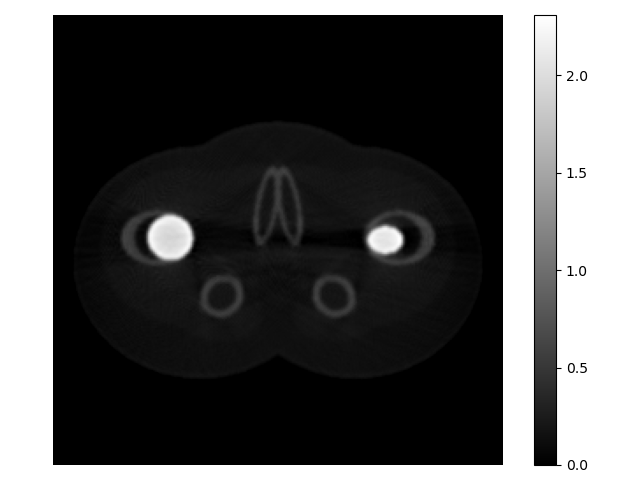
\includegraphics[width=\linewidth]{test_noise_ramlak.png}
        \caption{}
    \end{subfigure}
    \caption{Reconstructed images of bilateral hip replacement phantom under low mAs setting (100). (a) with only Ram-Lak filter, (b) with $\alpha=3$ raised cosine filter.}
    \label{fig:noise_ramlak}
\end{figure}
Using a Ram-Lak filter with suppressed high-frequency components ($\alpha > 1$) can effectively reduce streaking artefacts caused by scattering noise, as shown in Fig~\ref{fig:noise_ramlak}.
The raised cosine filter smooths reconstruction overall, thus removing visible streaks and granularity. However, it also reduces the resolution of the image and obscure finer details, which is a trade-off between noise reduction and image quality and should be balanced carefully according to each application.

\subsection{Beam Hardening Correction}
\vspace{-1em}
\begin{figure}[htbp]
    \centering
    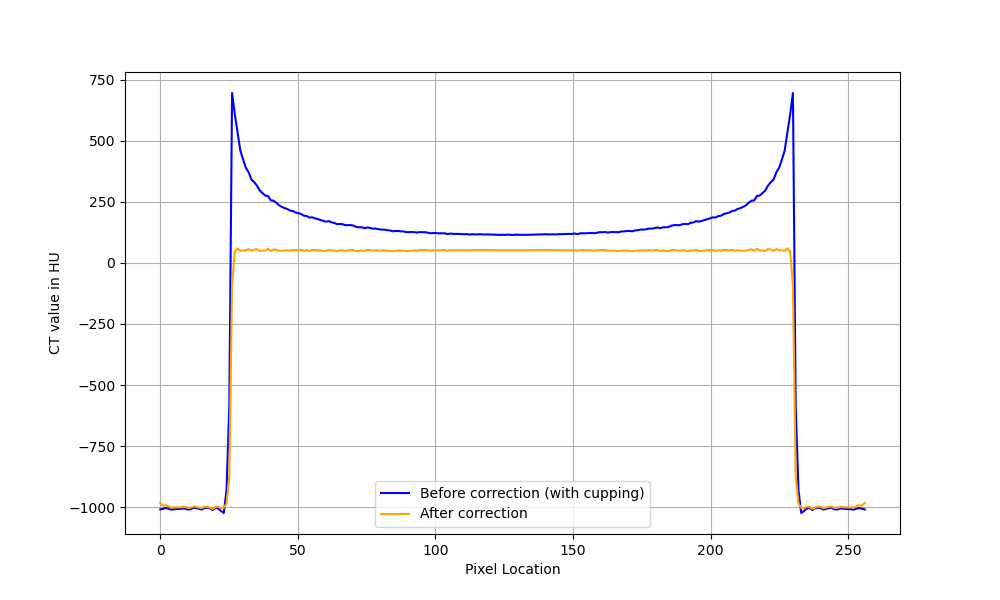
\includegraphics[width=\linewidth]{s712_beam_hardening on a slice.png}
    \caption{Beam hardening artefact in a slice of the reconstructed image of disk phantom before and after correction.}
    \label{fig:beam_hardening}
\end{figure}
Beam hardening occurs when lower-energy photons are attenuated more than higher-energy ones, due to the polychromatic X-ray spectrum, leading to a non-linear underestimation of attenuation. This causes the cupping artefact—reduced central attenuation compared to the edges—especially in high-density materials (Fig.\ref{fig:beam_hardening}).
Correction involves fitting a polynomial to attenuation profiles across water thicknesses to estimate a correction factor for the material. The corrected result is also shown in Fig.\ref{fig:beam_hardening}.

\subsection{Hounsfield Units (HU) Conversion}
HU is a standardised scale for quantifying X-ray attenuation subject to varations of source energy, which is defined as calibration against attenuation of water. Implementing HU conversion in the calibration process results in a HU value of $49.95$ for soft tissue under both real and ideal sources, which is consistent with the expected value of $50$ HU for soft tissue \cite{KIM20133}.

\section{Conclusion}
In this report, the process of simulating a CT scanner is documented, including scan generation, attenuation calculation, and reconstruction of the artificial cross-sectional data.
Future work is expected to include more refinements to the simulation, as well as in-depth investigation of specific applications of the simulator.

\begingroup
\scriptsize
\bibliographystyle{plain}
\bibliography{ref}
\endgroup
\end{document}